\section{Validacion Matematica Manual}
\label{sec:validacion}

Antes de medir tiempos es necesario comprobar que ambos algoritmos calculan correctamente los puntos de la curva. Para ello se calcula a mano una curva cubica en cinco valores del parametro, aplicando las Ecuaciones~\ref{eq:bernstein} y \ref{eq:casteljau} de la Seccion~\ref{sec:fundamentos}. Luego los resultados se comparan con los que entrega la aplicacion.

\subsection{Datos de la Prueba}
\label{subsec:val_datos}

Se usa una curva de grado $n = 3$ con los puntos de control del Cuadro~\ref{tab:val_puntos} y los valores $t \in \{0;\ 0.25;\ 0.5;\ 0.75;\ 1\}$, que equivalen a $N = 5$ muestras segun la Ecuacion~\ref{eq:fund_muestreo}.

\begin{table}[H]
\centering
\caption{Puntos de control de la curva cubica de prueba.}
\label{tab:val_puntos}
\begin{tabular}{ccc}
\toprule
\textbf{Punto} & \textbf{$x$} & \textbf{$y$} \\
\midrule
$P_0$ & $0$ & $0$ \\
$P_1$ & $1$ & $3$ \\
$P_2$ & $4$ & $3$ \\
$P_3$ & $5$ & $0$ \\
\bottomrule
\end{tabular}
\end{table}

\subsection{Calculo con Polinomios de Bernstein}
\label{subsec:val_bernstein}

Con la Ecuacion~\ref{eq:fund_binomial} se obtienen los coeficientes binomiales para $n = 3$:
\begin{equation}
\label{eq:val_binomiales}
\binom{3}{0} = 1, \quad
\binom{3}{1} = 1 \cdot \frac{3}{1} = 3, \quad
\binom{3}{2} = 3 \cdot \frac{2}{2} = 3, \quad
\binom{3}{3} = 3 \cdot \frac{1}{3} = 1
\end{equation}

Al reemplazarlos en la Ecuacion~\ref{eq:fund_base} quedan las cuatro bases cubicas:
\begin{equation}
\label{eq:val_bases_cubicas}
B_{0,3}(t) = (1-t)^3, \quad B_{1,3}(t) = 3t(1-t)^2, \quad B_{2,3}(t) = 3t^2(1-t), \quad B_{3,3}(t) = t^3
\end{equation}

\subsubsection{Ejemplo detallado para $t = 0.5$}

Se evalua cada base con $t = 0.5$ y $1 - t = 0.5$:
\begin{align}
B_{0,3}(0.5) & = 1 \cdot 0.5^3 \cdot 0.5^0 = 0.125 \nonumber \\
B_{1,3}(0.5) & = 3 \cdot 0.5^2 \cdot 0.5^1 = 0.375 \nonumber \\
B_{2,3}(0.5) & = 3 \cdot 0.5^1 \cdot 0.5^2 = 0.375 \nonumber \\
B_{3,3}(0.5) &= 1 \cdot 0.5^0 \cdot 0.5^3 = 0.125 \label{eq:val_bases_t05}
\end{align}

Las cuatro bases suman $0.125 + 0.375 + 0.375 + 0.125 = 1$, lo que confirma la particion de la unidad. Luego se calcula la suma ponderada de cada coordenada:
\begin{align}
x(0.5) & = 0.125(0) + 0.375(1) + 0.375(4) + 0.125(5) = 0 + 0.375 + 1.5 + 0.625 = 2.5 \nonumber \\
y(0.5) &= 0.125(0) + 0.375(3) + 0.375(3) + 0.125(0) = 0 + 1.125 + 1.125 + 0 = 2.25 \label{eq:val_bernstein_t05}
\end{align}

Por lo tanto, $C(0.5) = (2.5;\ 2.25)$.

\subsubsection{Resultados para todos los valores de $t$}

El mismo procedimiento se repite para los cinco valores del parametro. En el Cuadro~\ref{tab:val_bases} se muestran los valores de las bases y el punto resultante. En $t = 0$ y $t = 1$ se aplica la convencion $0^0 = 1$ descrita en la Seccion~\ref{sec:fundamentos}.

\begin{table}[H]
\centering
\caption{Valores de las bases de Bernstein y puntos de la curva cubica de prueba.}
\label{tab:val_bases}
\begin{tabular}{c cccc c}
\toprule
\textbf{$t$} & \textbf{$B_{0,3}$} & \textbf{$B_{1,3}$} & \textbf{$B_{2,3}$} & \textbf{$B_{3,3}$} & \textbf{$C(t) = (x, y)$} \\
\midrule
$0.00$ & $1.000000$ & $0.000000$ & $0.000000$ & $0.000000$ & $(0.0000;\ 0.0000)$ \\
$0.25$ & $0.421875$ & $0.421875$ & $0.140625$ & $0.015625$ & $(1.0625;\ 1.6875)$ \\
$0.50$ & $0.125000$ & $0.375000$ & $0.375000$ & $0.125000$ & $(2.5000;\ 2.2500)$ \\
$0.75$ & $0.015625$ & $0.140625$ & $0.421875$ & $0.421875$ & $(3.9375;\ 1.6875)$ \\
$1.00$ & $0.000000$ & $0.000000$ & $0.000000$ & $1.000000$ & $(5.0000;\ 0.0000)$ \\
\bottomrule
\end{tabular}
\end{table}

\subsection{Calculo con el Algoritmo de De Casteljau}
\label{subsec:val_casteljau}

\subsubsection{Ejemplo detallado para $t = 0.5$}

Se aplica la Ecuacion~\ref{eq:casteljau} nivel por nivel. Con $t = 0.5$ cada interpolacion equivale al punto medio entre dos puntos consecutivos.

\textbf{Nivel 1} ($r = 1$, tres puntos):
\begin{align}
P_0^{(1)} & = 0.5(0;\ 0) + 0.5(1;\ 3) = (0.5;\ 1.5) \nonumber \\
P_1^{(1)} & = 0.5(1;\ 3) + 0.5(4;\ 3) = (2.5;\ 3.0) \nonumber \\
P_2^{(1)} &= 0.5(4;\ 3) + 0.5(5;\ 0) = (4.5;\ 1.5) \label{eq:val_nivel1}
\end{align}

\textbf{Nivel 2} ($r = 2$, dos puntos):
\begin{align}
P_0^{(2)} & = 0.5(0.5;\ 1.5) + 0.5(2.5;\ 3.0) = (1.5;\ 2.25) \nonumber \\
P_1^{(2)} &= 0.5(2.5;\ 3.0) + 0.5(4.5;\ 1.5) = (3.5;\ 2.25) \label{eq:val_nivel2}
\end{align}

\textbf{Nivel 3} ($r = 3$, un punto):
\begin{equation}
\label{eq:val_nivel3}
P_0^{(3)} = 0.5(1.5;\ 2.25) + 0.5(3.5;\ 2.25) = (2.5;\ 2.25)
\end{equation}

El resultado $C(0.5) = (2.5;\ 2.25)$ coincide con el obtenido por Bernstein en la Ecuacion~\ref{eq:val_bernstein_t05}. La Figura~\ref{fig:val_casteljau_t05} muestra esta construccion geometrica.

\begin{figure}[H]
\centering
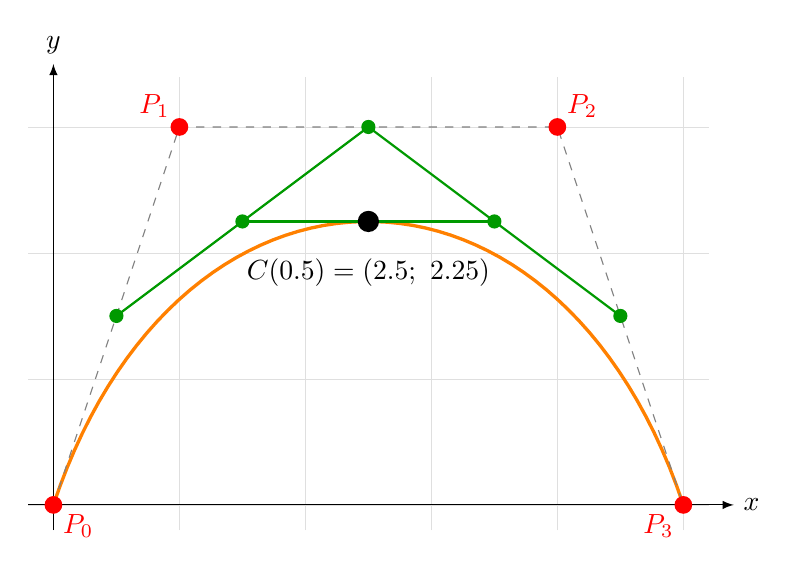
\begin{tikzpicture}[scale=1.6]
  % Cuadricula y ejes
  \draw[gray!25, very thin] (-0.2,-0.2) grid (5.2,3.4);
  \draw[-latex] (-0.2,0) -- (5.4,0) node[right] {$x$};
  \draw[-latex] (0,-0.2) -- (0,3.5) node[above] {$y$};
  % Curva cubica evaluada con la forma de Bernstein (parametro \x = t)
  \draw[very thick, orange, domain=0:1, samples=60]
    plot ({3*\x*(1-\x)^2*1 + 3*\x^2*(1-\x)*4 + \x^3*5}, {3*\x*(1-\x)^2*3 + 3*\x^2*(1-\x)*3});
  % Poligono de control (nivel 0)
  \draw[dashed, gray] (0,0) -- (1,3) -- (4,3) -- (5,0);
  % Nivel 1 y nivel 2
  \draw[green!60!black, thick] (0.5,1.5) -- (2.5,3) -- (4.5,1.5);
  \draw[green!60!black, thick] (1.5,2.25) -- (3.5,2.25);
  % Puntos de control
  \foreach \px/\py/\nom/\pos in {0/0/P_0/below right, 1/3/P_1/above left, 4/3/P_2/above right, 5/0/P_3/below left} {
    \fill[red] (\px,\py) circle (2pt) node[\pos, red] {$\nom$};
  }
  % Puntos intermedios
  \foreach \px/\py in {0.5/1.5, 2.5/3, 4.5/1.5, 1.5/2.25, 3.5/2.25} {
    \fill[green!60!black] (\px,\py) circle (1.6pt);
  }
  % Punto de la curva
  \fill[black] (2.5,2.25) circle (2.4pt) node[below=10pt] {$C(0.5) = (2.5;\ 2.25)$};
\end{tikzpicture}
\caption{Construccion de De Casteljau para $t = 0.5$: poligono de control (gris), niveles intermedios (verde) y punto de la curva (negro).}
\label{fig:val_casteljau_t05}
\end{figure}

\subsubsection{Niveles para todos los valores de $t$}

El Cuadro~\ref{tab:val_niveles} resume los puntos de cada nivel para los cinco valores del parametro. El ultimo nivel contiene el punto de la curva.

\begin{table}[H]
\centering
\caption{Niveles intermedios de De Casteljau para la curva cubica de prueba.}
\label{tab:val_niveles}
\small
\setlength{\tabcolsep}{4pt}
\begin{tabular}{c ccc cc c}
\toprule
\textbf{$t$} & \textbf{$P_0^{(1)}$} & \textbf{$P_1^{(1)}$} & \textbf{$P_2^{(1)}$} & \textbf{$P_0^{(2)}$} & \textbf{$P_1^{(2)}$} & \textbf{$P_0^{(3)} = C(t)$} \\
\midrule
$0.00$ & $(0;\ 0)$ & $(1;\ 3)$ & $(4;\ 3)$ & $(0;\ 0)$ & $(1;\ 3)$ & $(0;\ 0)$ \\
$0.25$ & $(0.25;\ 0.75)$ & $(1.75;\ 3)$ & $(4.25;\ 2.25)$ & $(0.625;\ 1.3125)$ & $(2.375;\ 2.8125)$ & $(1.0625;\ 1.6875)$ \\
$0.50$ & $(0.5;\ 1.5)$ & $(2.5;\ 3)$ & $(4.5;\ 1.5)$ & $(1.5;\ 2.25)$ & $(3.5;\ 2.25)$ & $(2.5;\ 2.25)$ \\
$0.75$ & $(0.75;\ 2.25)$ & $(3.25;\ 3)$ & $(4.75;\ 0.75)$ & $(2.625;\ 2.8125)$ & $(4.375;\ 1.3125)$ & $(3.9375;\ 1.6875)$ \\
$1.00$ & $(1;\ 3)$ & $(4;\ 3)$ & $(5;\ 0)$ & $(4;\ 3)$ & $(5;\ 0)$ & $(5;\ 0)$ \\
\bottomrule
\end{tabular}
\end{table}

\subsection{Verificacion con la Aplicacion}
\label{subsec:val_verificacion}

Para confirmar los calculos manuales se ejecuto el proyecto de consola de prueba manual del repositorio:
\begin{center}
\texttt{src/BezierComparador.PruebaManual}
\end{center}
Este proyecto usa directamente las clases del Modelo, es decir, los dos evaluadores y el comparador numerico, y muestra el mismo procedimiento paso a paso. La salida completa se encuentra en el Anexo~\ref{subsec:anx_salida} y una captura de su ejecucion en la Figura~\ref{fig:val_consola}.

\begin{table}[H]
\centering
\caption{Comparacion del calculo manual con los resultados de la aplicacion.}
\label{tab:val_comparacion}
\begin{tabular}{c cc c}
\toprule
\textbf{$t$} & \textbf{Bernstein (aplicacion)} & \textbf{De Casteljau (aplicacion)} & \textbf{Diferencia $d$} \\
\midrule
$0.00$ & $(0.000000;\ 0.000000)$ & $(0.000000;\ 0.000000)$ & $0$ \\
$0.25$ & $(1.062500;\ 1.687500)$ & $(1.062500;\ 1.687500)$ & $0$ \\
$0.50$ & $(2.500000;\ 2.250000)$ & $(2.500000;\ 2.250000)$ & $0$ \\
$0.75$ & $(3.937500;\ 1.687500)$ & $(3.937500;\ 1.687500)$ & $0$ \\
$1.00$ & $(5.000000;\ 0.000000)$ & $(5.000000;\ 0.000000)$ & $0$ \\
\bottomrule
\end{tabular}
\end{table}

\capturaPendiente{0.9\textwidth}{7cm}{Salida por consola del proyecto BezierComparador.PruebaManual con el calculo paso a paso de ambos metodos.}{fig:val_consola}

Como se observa en el Cuadro~\ref{tab:val_comparacion}, los valores de la aplicacion coinciden con los calculados a mano, y la diferencia entre ambos metodos es exactamente cero en los cinco valores de $t$. Esto ocurre porque los puntos de control son enteros y los valores de $t$ son fracciones con denominador potencia de dos ($1/4$, $1/2$, $3/4$). Todos los resultados intermedios pueden representarse de forma exacta en punto flotante binario, por lo que no se produce error de redondeo. Con otros valores de $t$ o con grados mayores aparecen diferencias pequenas, que se analizan en la Seccion~\ref{sec:comparacion}.

Tambien se observa que la curva es simetrica respecto a la recta $x = 2.5$, ya que los puntos de control son simetricos: $C(0.25)$ y $C(0.75)$ tienen la misma altura $y = 1.6875$. Esta validacion confirma que ambas implementaciones son correctas antes de pasar a la experimentacion.

% RESUMEN: Esta seccion (03_validacion_manual.tex) calcula a mano la curva cubica
% P0=(0;\ 0) P1=(1;\ 3) P2=(4;\ 3) P3=(5;\ 0) en t = 0, 0.25, 0.5, 0.75, 1 con Bernstein
% (tab:val_bases) y De Casteljau (tab:val_niveles), con el ejemplo detallado en t = 0.5,
% la figura TikZ fig:val_casteljau_t05 y la comparacion con la aplicacion
% (tab:val_comparacion). Todos los valores salen de validacion_manual.txt, generado por
% el proyecto BezierComparador.PruebaManual. Captura pendiente: fig:val_consola
% (archivo figuras/val_consola.png). Etiqueta principal: sec:validacion.
% Referencia \ref{subsec:anx_salida} de 08_anexos.tex.
